% Created 2016-06-07 Tue 13:58
\documentclass[presentation]{beamer}
\usepackage[utf8]{inputenc}
\usepackage[T1]{fontenc}
\usepackage{fixltx2e}
\usepackage{graphicx}
\usepackage{grffile}
\usepackage{longtable}
\usepackage{wrapfig}
\usepackage{rotating}
\usepackage[normalem]{ulem}
\usepackage{amsmath}
\usepackage{textcomp}
\usepackage{amssymb}
\usepackage{capt-of}
\usepackage{hyperref}
\usetheme{Frankfurt}
\usecolortheme{}
\usefonttheme{}
\useinnertheme{}
\useoutertheme{}
\author{Daniel Kessler}
\date{\textit{<2016-06-08 Wed>}}
\title{Growth Charting of Brain Connectivity Networks and the Identification of Attention Impairment in Youth}
\subtitle{Published in JAMA Psychiatry, 2016 (Kessler, Sripada, \& Angstadt)}

\hypersetup{
 pdfauthor={Daniel Kessler},
 pdftitle={Growth Charting of Brain Connectivity Networks and the Identification of Attention Impairment in Youth},
 pdfkeywords={},
 pdfsubject={},
 pdfcreator={Emacs 24.3.1 (Org mode 8.3.4)}, 
 pdflang={English}}
\begin{document}

\maketitle
\begin{frame}{Outline}
\tableofcontents
\end{frame}




\section{Introduction}
\label{sec:orgheadline3}
\stepcounter{subsection}
\begin{frame}[label={sec:orgheadline1}]{Motivation}
\begin{block}{Pediatric Growth Charts}
\begin{itemize}
\item Long history for height, weight, etc
\end{itemize}
\end{block}
\begin{block}{Intrinsic Connectivity Networks}
\begin{itemize}
\item Attention \& ADHD connection
\item DMN vs TPN balance
\end{itemize}
\end{block}
\end{frame}
\begin{frame}[label={sec:orgheadline2}]{Background}
Focus today: processing pipeline, modeling, and analysis
\end{frame}
\section{Methods}
\label{sec:orgheadline18}
\stepcounter{subsection}
\begin{frame}[label={sec:orgheadline4}]{Sample}
\begin{itemize}
\item Philadelphia Neurodevelopmental Cohort
\item Resting state fMRI
\item Penn Continuous Performance Task
\item N = 519 (after QC \& exclusions)
\end{itemize}
\end{frame}
\begin{frame}[label={sec:orgheadline5}]{Task: PCPT}
\begin{itemize}
\item Penn Continuous Performance Test
\item 180 trials
\item 1s to respond
\item "Go" on digit/letter (varies by phase)
\item Measure: Acc (as \%age)
\end{itemize}
\end{frame}
\begin{frame}[label={sec:orgheadline6}]{Clinical Interview}
\end{frame}
\begin{frame}[label={sec:orgheadline7}]{MRI Measures}
\begin{itemize}
\item T1-weighted image (structural contrast)
\item Resting State fMRI
\end{itemize}
\end{frame}
\begin{frame}[label={sec:orgheadline8}]{Standard fMRI Prepocessing}
\begin{enumerate}
\item Slice-time Correction
\item Motion Correction
\item Normalization
\item Smoothing
\end{enumerate}
\end{frame}
\begin{frame}[label={sec:orgheadline9}]{Slice-time Correction}
\begin{columns}
\begin{column}{.2\columnwidth}
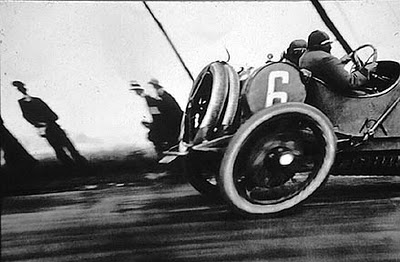
\includegraphics[width=3cm]{/home/kesslerd/OrgMode/Work/jICA_JAMA_Presentation/rollingshuttercar.jpg}
\end{column}
\begin{column}{.5\columnwidth}
\begin{itemize}
\item Each fMRI volume is acquired sequentially in slices
\item Volume not acquired simultaneously
\item Correct (through interpolation) s.t. all slices w/in volume temporally aligned
\end{itemize}
\end{column}
\end{columns}
\end{frame}
\begin{frame}[label={sec:orgheadline10}]{Motion Correction}
\begin{itemize}
\item Participants move their head over the scan
\end{itemize}
\end{frame}
\begin{frame}[label={sec:orgheadline11}]{Normalization}
\end{frame}
\begin{frame}[label={sec:orgheadline12}]{Smoothing}
\end{frame}

\begin{frame}[label={sec:orgheadline13}]{Preprocessing \& Connectome Generation}
\begin{block}{Preprocessing}
\begin{itemize}
\item Linearly detrended
\item COMPCor
\item Bandpass Filtering
\item Motion Scrubbing
\end{itemize}
\end{block}
\begin{block}{Connectome Generation}
\begin{itemize}
\item Isomorphic grid
\item 12mm spacing
\item 

\item 1068 Regions of Interest (ROIs)
\end{itemize}
\end{block}
\end{frame}
\begin{frame}[label={sec:orgheadline14}]{Data Cleansing}
\end{frame}
\begin{frame}[label={sec:orgheadline15}]{Preprocessing \& Connectome Generation}
\end{frame}
\begin{frame}[label={sec:orgheadline16}]{Independent Components Analysis}
\end{frame}
\begin{frame}[label={sec:orgheadline17}]{Network Growth Charting Analyses}
\end{frame}
\section{Results}
\label{sec:orgheadline24}
\stepcounter{subsection}
\begin{frame}[label={sec:orgheadline19}]{Network Growth Charting to Predict Task Accuracy}
\end{frame}
\begin{frame}[label={sec:orgheadline20}]{Shifting DMN-TPN Architecture Among Maturing Components}
\end{frame}
\begin{frame}[label={sec:orgheadline21}]{Shallow vs Lagged Dysmaturation and Task Accuracy}
\end{frame}
\begin{frame}[label={sec:orgheadline22}]{Biomarker of Attention Dysfunction from Network Growth Charting}
\end{frame}
\begin{frame}[label={sec:orgheadline23}]{Biomarker of ADHD from Network Growth Charting}
\end{frame}
\section{Discussion}
\label{sec:orgheadline29}
\stepcounter{subsection}
\begin{frame}[label={sec:orgheadline25}]{Unraveling miswired connectomes}
\end{frame}
\begin{frame}[label={sec:orgheadline26}]{ICN interplay}
\end{frame}
\begin{frame}[label={sec:orgheadline27}]{Dysmaturation Predicts Dysfunction}
\end{frame}
\begin{frame}[label={sec:orgheadline28}]{Differential Dysmaturation}
\end{frame}
\section{Conclusions}
\label{sec:orgheadline31}
\stepcounter{subsection}
\begin{frame}[label={sec:orgheadline30}]{Conclusions}
Brain network growth charting predicts attention functioning.
\end{frame}
\end{document}
